\begin{figure}[H]
\centering
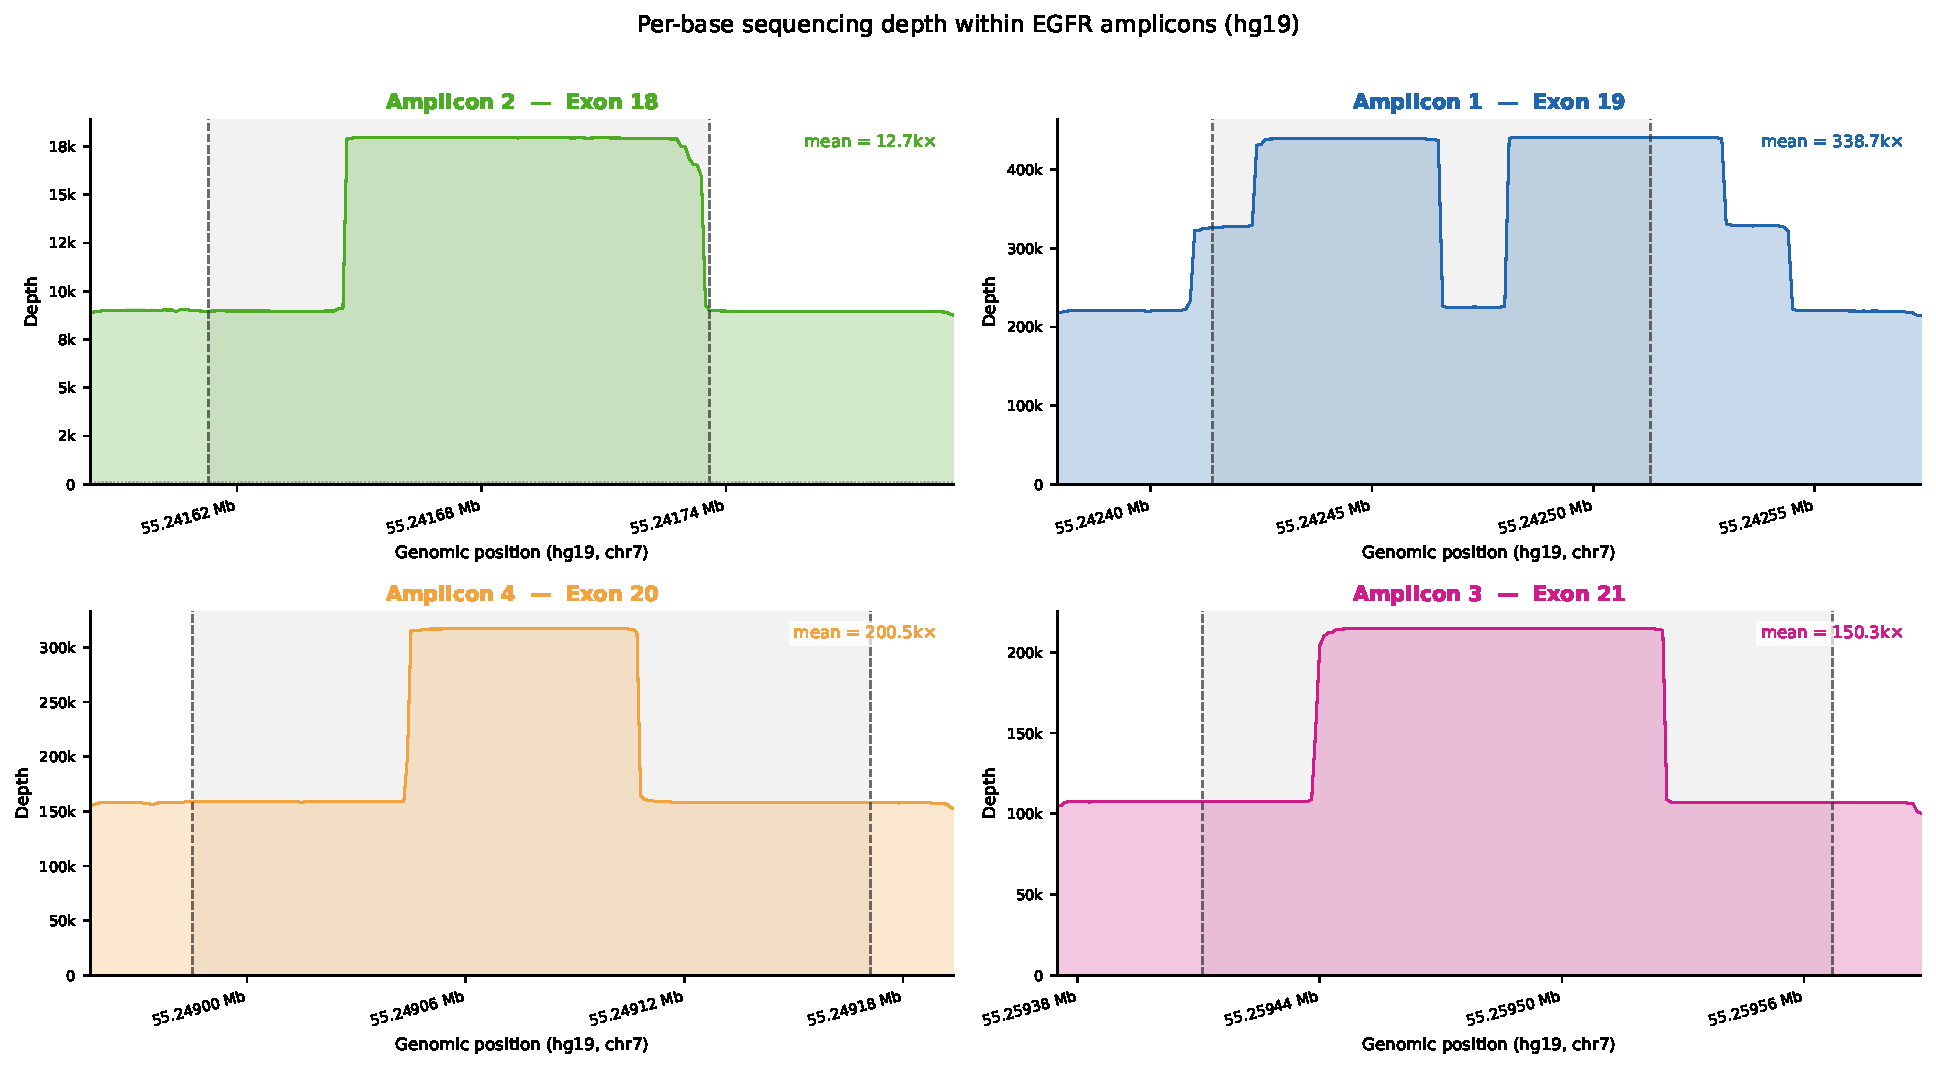
\includegraphics[width=\textwidth]{figures/amplicon_depth_plot.pdf}
\caption{Per-base sequencing depth within each EGFR amplicon (hg19, chr7).
Grey shading marks the target exon; dashed vertical lines indicate the exon
boundaries. The depth step-up inside the exon relative to the flanking
intronic primer regions is expected: intronic positions are covered by reads
from one direction only (R1 or R2), whereas the exon --- where R1 and R2
overlap --- is covered by reads from both directions, approximately doubling
the local depth.
Summary statistics (computed from \texttt{mapping/amplicon\_depth\_annotated.txt}):
all four amplicons achieve 100\% of bases at $\geq$10$\times$ and $\geq$100$\times$ coverage.
Mean depths are: Amplicon~2 (Ex18) 12{,}650$\times$;
Amplicon~1 (Ex19) 338{,}664$\times$; Amplicon~4 (Ex20) 200{,}484$\times$;
Amplicon~3 (Ex21) 150{,}290$\times$.
The notably lower depth of Amplicon~2 relative to the other three amplicons
is discussed in the uniformity analysis (Section~\ref{sec:coverage-uniformity}).}
\label{fig:amplicon-depth}
\end{figure}
